\chapter{TP2:Utilisation du CAN de l’Arduino}
\minitoc
\newpage
\section{Convertisseur Analogique numérique}
La carte Arduino Uno intègre un unique convertisseur analogique/numérique (CAN) de 10 bits, partagé entre ses 6 entrées (A0 à A5). Il convertit le signal en environ 100 µs pour délivrer une valeur numérique allant de 0 à 1023.
\section{Mesurer une température avec un capteur LM35 et une carte Arduino}
Le LM35 est un capteur de température électronique analogique de précision. Il se présente sous la forme d'un composant à trois broches :
\begin{itemize}
	\item \textbf{VCC} : Alimentation (reliée au 5V)
	\item \textbf{Analog Voltage Out} : Sortie de la tension (reliée à une entrée analogique)
	\item \textbf{GND} : Masse
\end{itemize}
\paragraph{Principe de mesure :}
D'après la fiche technique du composant, la tension de sortie est proportionnelle à la température avec une sensibilité de $10\,\mathrm{mV} / ^{\circ}\mathrm{C}$. Autrement dit, une tension de $1\,\mathrm{V}$ correspond à $100^{\circ}\mathrm{C}$.\\
\begin{figure}[H]
	\centering
	\begin{minipage}{0.48\textwidth}
		\centering
		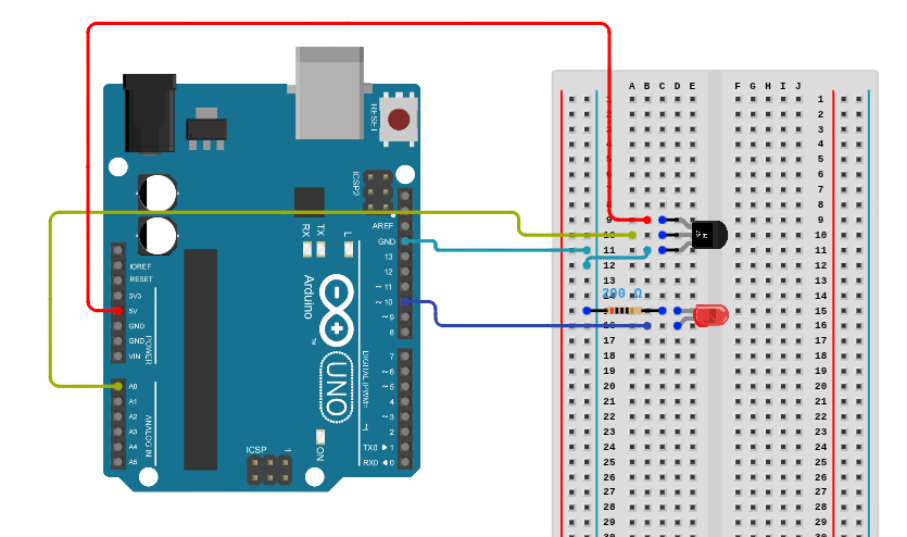
\includegraphics[width=\linewidth]{Image/2.maniptempérature}
		\caption{Schéma de l'utilisation du LM35}
		\label{fig:schema_lm35}
	\end{minipage}\hfill
	\begin{minipage}{0.48\textwidth}
		\centering
		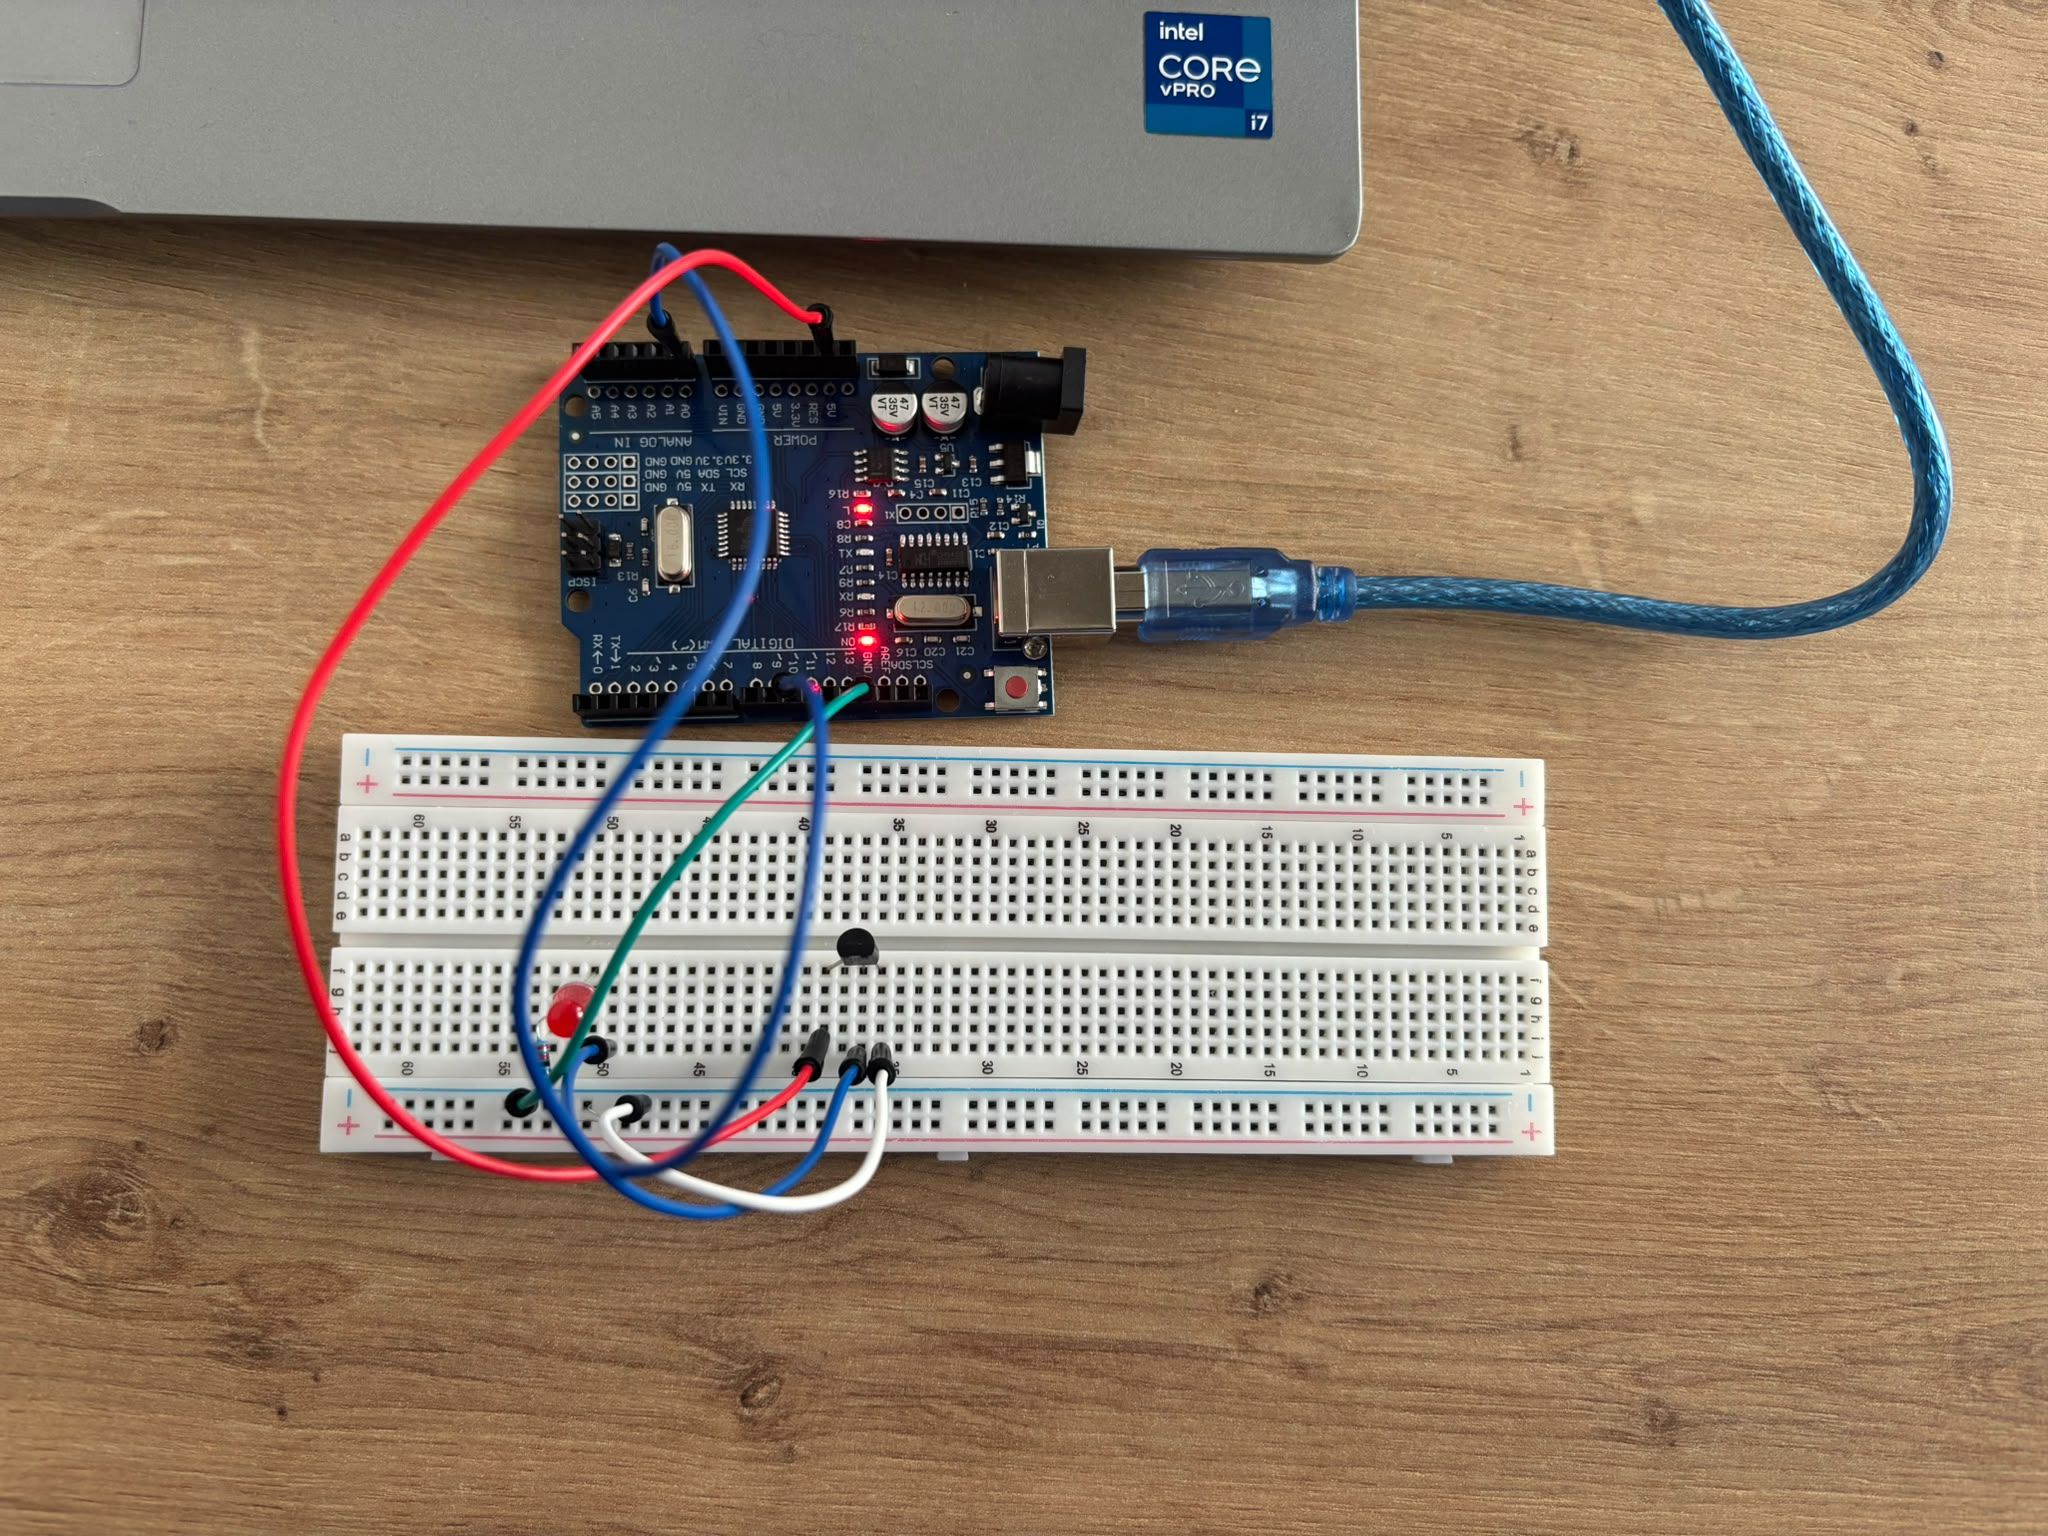
\includegraphics[width=\linewidth]{Image/2.Photomainp_température}
		\caption{Photo du montage du LM35}
		\label{fig:photo_lm35}
	\end{minipage}
\end{figure}
Pour commencer nous allons programmer la carte pour uniquement récupérer les informations du LM35.
\begin{lstlisting}				
const int lm35Pin = A0; // Broche du capteur LM35

void setup() {
	Serial.begin(9600); // Initialisation de la communication serie
}
void loop() {
	int val = analogRead(lm35Pin); // Lecture de la valeur analogique (0 a 1023)
	
	// Conversion de la valeur lue en tension (en mV), puis en temperature (C)
	
	float voltage = val * (5.0 / 1023.0);
	float temperature = voltage * 100.0; // 10 mV par C donc T = tension * 100
	
	Serial.print("Temperature : ");
	Serial.print(temperature);
	Serial.println(" C");
	
	delay(1000); // Pause d'une seconde entre chaque mesure
}
\end{lstlisting}
\textbf{Observations :} Nous utilisons le moniteur série de l'Arduino pour relever la température mesurée par le capteur. La valeur obtenue étant d'environ 22 °C, nous pouvons en déduire que le montage et la programmation ont été réalisés avec succès.
\begin{figure}[H]
	\centering
	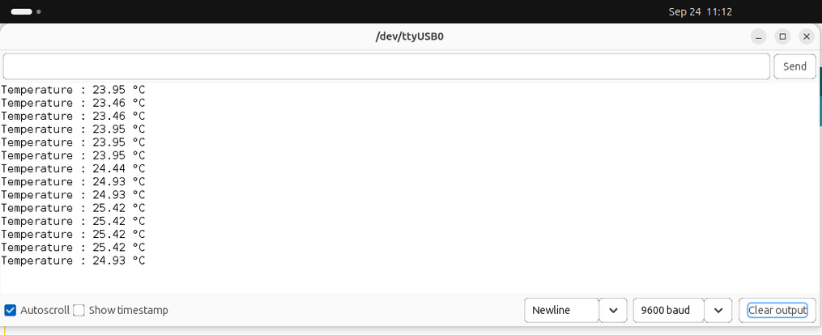
\includegraphics[width=0.7\linewidth]{Image/2.Resultat_LM35}
	\caption{Monitor série du capteur LM35}
	\label{fig:2}
\end{figure}
Nous faisons évoluer le programme pour utiliser la LED comme indicateur d'alerte. Si la température mesurée par le LM35 est supérieure à 35 °C, nous commandons l'allumage de la LED.
\begin{lstlisting}				
const int lm35Pin = A0; // Broche du capteur LM35
void setup() {
	Serial.begin(9600); // Initialisation de la communication serie
	pinMode(10, OUTPUT);
}
void loop() {
	int val = analogRead(lm35Pin); // Lecture de la valeur analogique (0 a 1023)

	// Conversion de la valeur lue en tension (en mV), puis en temperature (C)
	
	float voltage = val * (5.0 / 1023.0);
	float temperature = voltage * 100.0; // 10 mV par C donc T = tension * 100
	
	Serial.print("Temperature : ");
	Serial.print(temperature);
	Serial.println(" C");
	
	delay(1000); // Pause d'une seconde entre chaque mesure
	
	if (temperature > 29) {
		digitalWrite(10,HIGH); // on allume la LED
	}else {
		digitalWrite(10,LOW); // on eteint la LED
	}
}
\end{lstlisting}
\textbf{Observations :} Lorsque que nous plaçons notre doigts sur le LM35 alors la LED s'allume car nous dépassons le seuil de température de notre programme.
\section{Mesurer la luminosité avec une photorésistance et une carte Arduino}
Une \textbf{photorésistance} est un composant électronique dont la valeur (en ohms) varie en fonction de la lumière ambiante : \textbf{plus elle est éclairée, plus sa résistance diminue}.

\paragraph{Caractéristiques classiques}
\begin{itemize}
	\item \textbf{Dans l'obscurité :} Résistance très élevée (environ 1 M$\Omega$).
	\item \textbf{En pleine lumière :} Résistance plus faible (environ 12 k$\Omega$).
\end{itemize}

\paragraph{Applications principales}
Ce comportement permet de mesurer la luminosité ambiante pour diverses utilisations :
\begin{itemize}
	\item Détection de l'état jour/nuit.
	\item Ajustement automatique de l'éclairage.
	\item Systèmes de suivi de lumière (panneaux solaires, robotique).
\end{itemize}
\begin{figure}[H]
	\centering
	\begin{minipage}{0.48\textwidth}
		\centering
		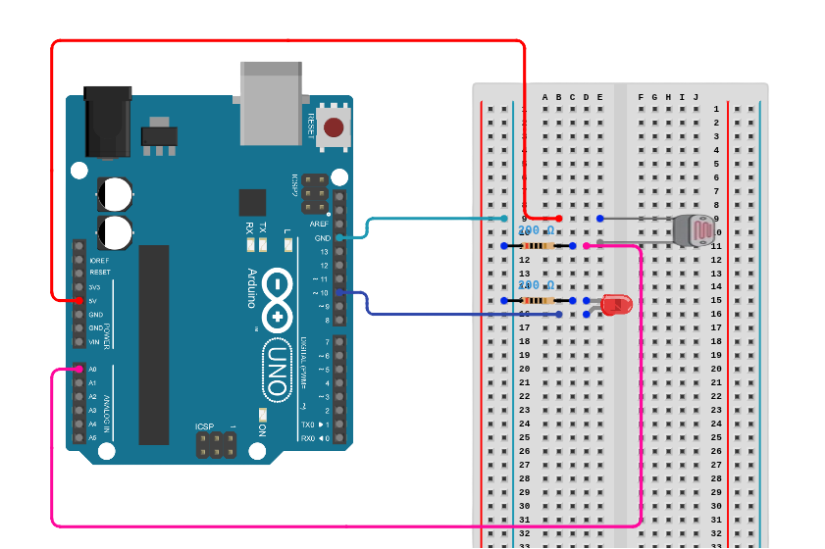
\includegraphics[width=\linewidth]{Image/2.Schéma_Manip2}
		\caption{Schéma du montage avec photorésistance}
		\label{fig:schema_photores}
	\end{minipage}\hfill
	\begin{minipage}{0.48\textwidth}
		\centering
		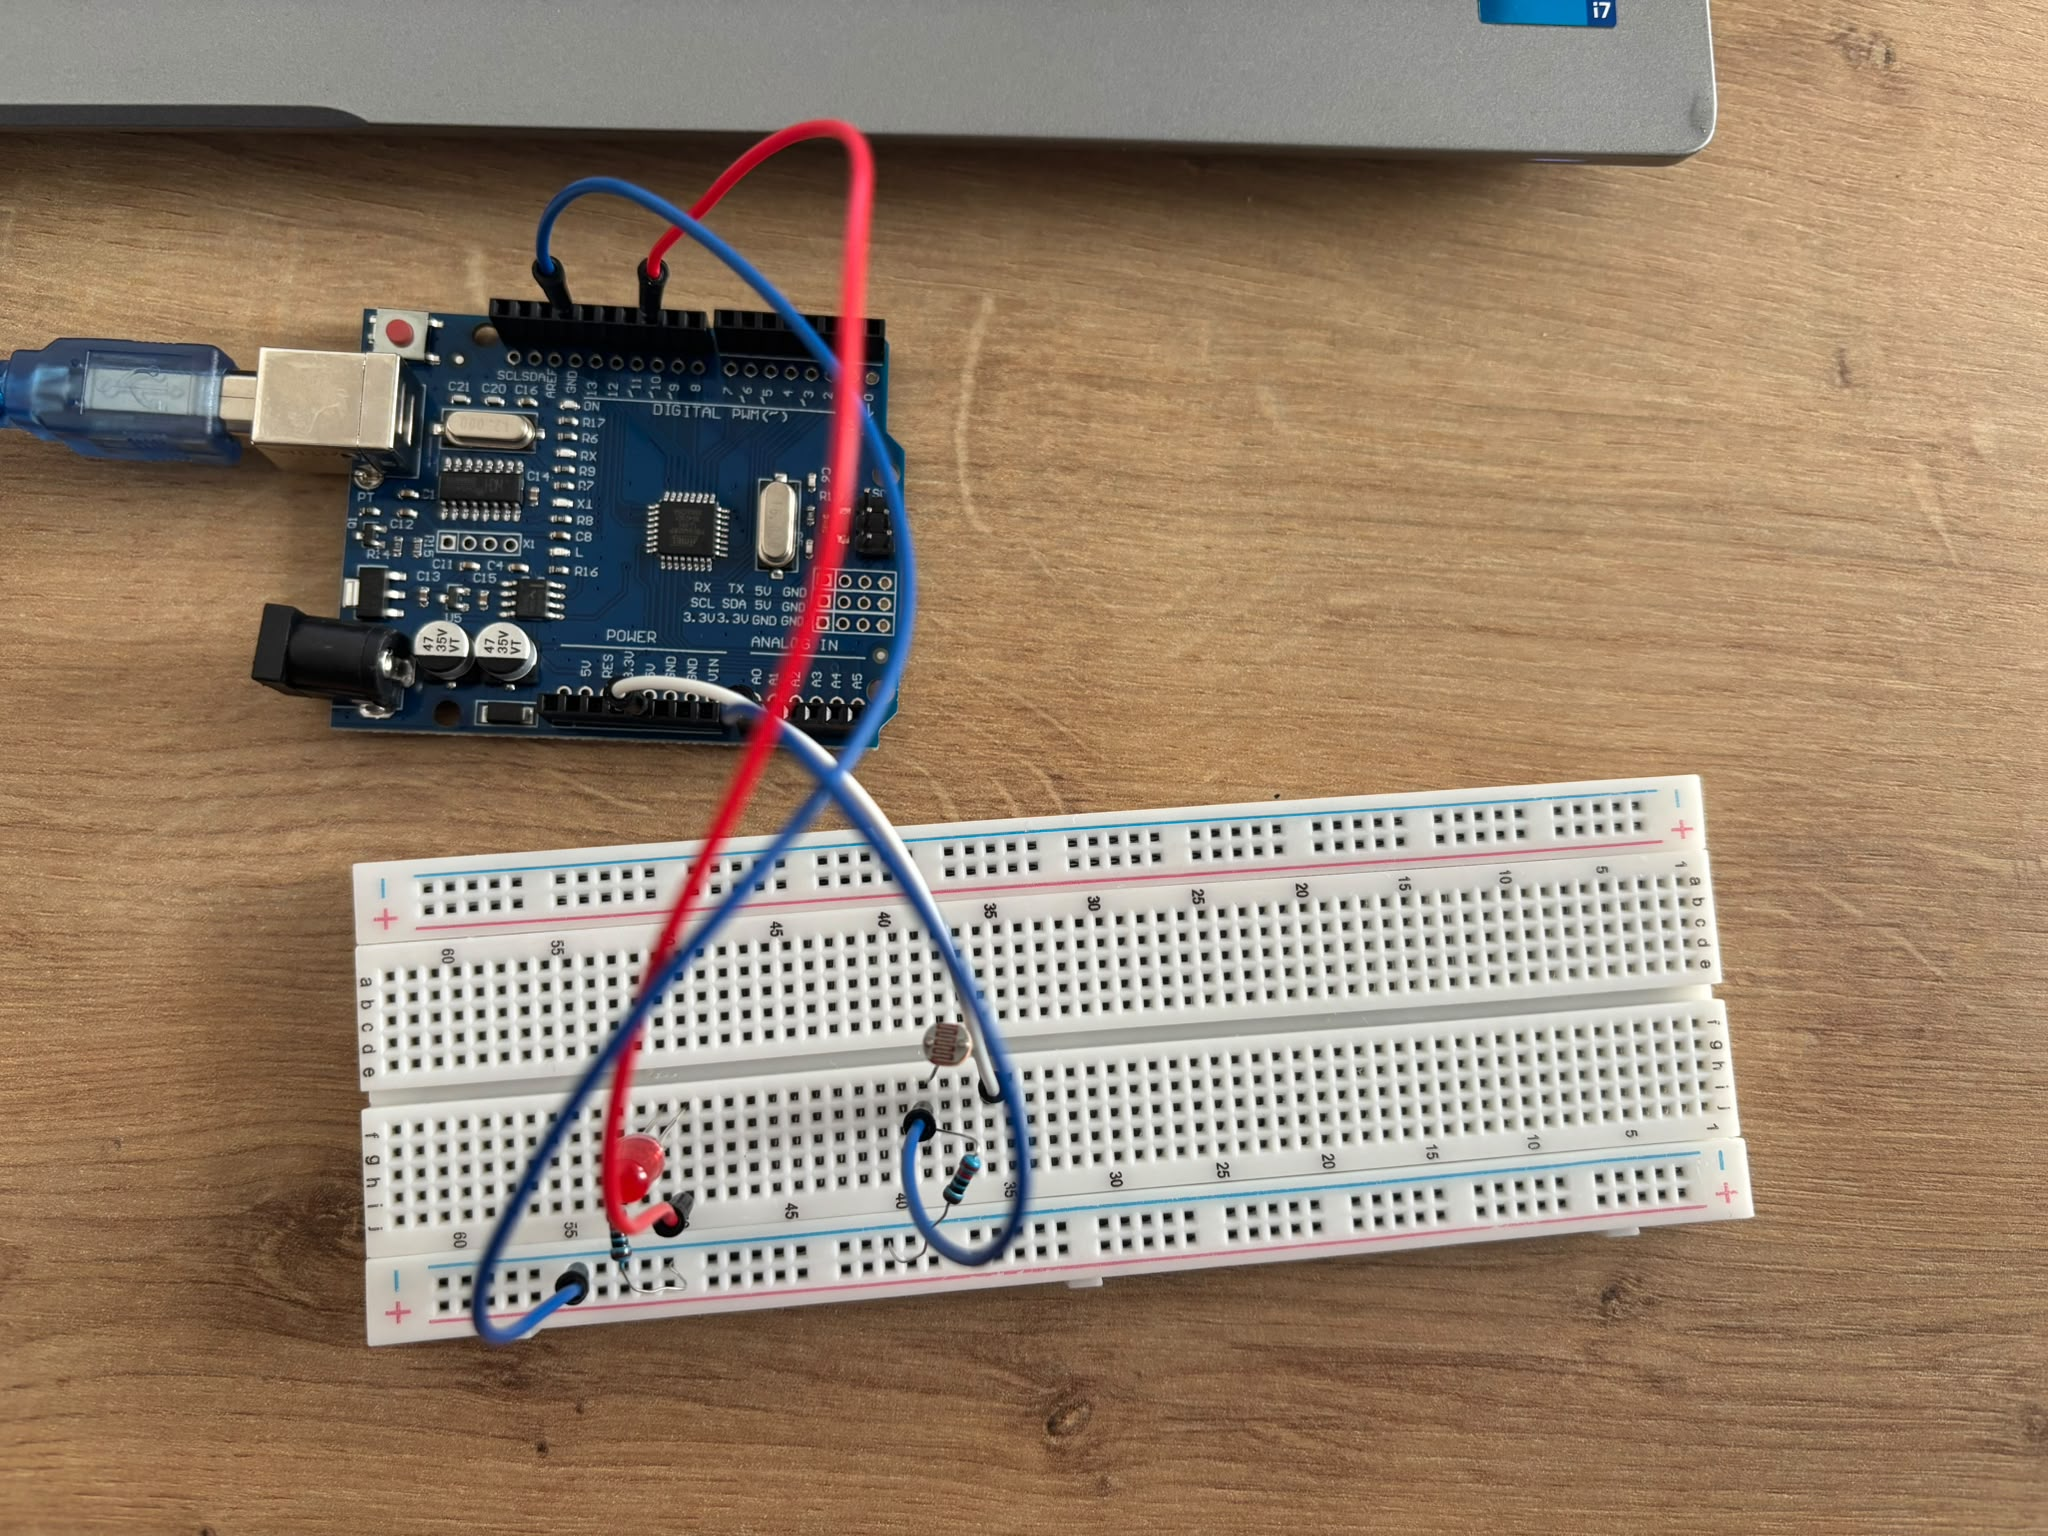
\includegraphics[width=\linewidth]{Image/2.Photo_Manip2}
		\caption{Photo montage avec la photorésistance}
		\label{fig:photo_photores}
	\end{minipage}
\end{figure}
Ensuite, nous allons faire un programme permettant de gérer l'allumage d'une LED en fonction de la luminosité reçue par la photorésistance.
\begin{lstlisting}					
	// Initialisation des constantes :
	const int analogInPin = A0; // Numero de la broche a laquelle est connectee la photoresistance
	const int analogOutPin = 10; // Numero de la broche a laquelle est connectee la LED
	
	int sensorValue = 0; // Valeur lue sur la photoresistance
	int outputValue = 0; // Valeur envoyee a la LED	
	void setup() {
		// Initialise la communication avec l'ordinateur
		Serial.begin(9600);
		// Indique que la broche analogOutPin est une sortie :
		pinMode(analogOutPin, OUTPUT);
		// Indique que la broche analogInPin est une entree :
		pinMode(analogInPin, INPUT);
	}	
	void loop() {
		// lit la valeur de la photoresistance et
		// stocke le resultat dans sensorValue :
		sensorValue = analogRead(analogInPin);
		// change sensorValue vers une intervalle de 0 a 255
		// et stocke le resultat dans outputValue :
		outputValue = map(sensorValue, 0, 1023, 0, 255);
		// envoie de cette nouvelle valeur sur la LED
		analogWrite(analogOutPin, outputValue);
		Serial.print("sensor = " );
		Serial.print(sensorValue);
		Serial.print("\t output = ");
		Serial.println(outputValue);
	}
\end{lstlisting}
\textbf{Observations :} Lorsque nous mettons notre doigt sur la photorésistance pour baiser la luminosité alors la LED s'allume.
Nous allons rajouter une autre LED qui s'allume avec un autre seuil.
\begin{figure}[H]
	\centering
	\begin{minipage}{0.48\textwidth}
		\centering
		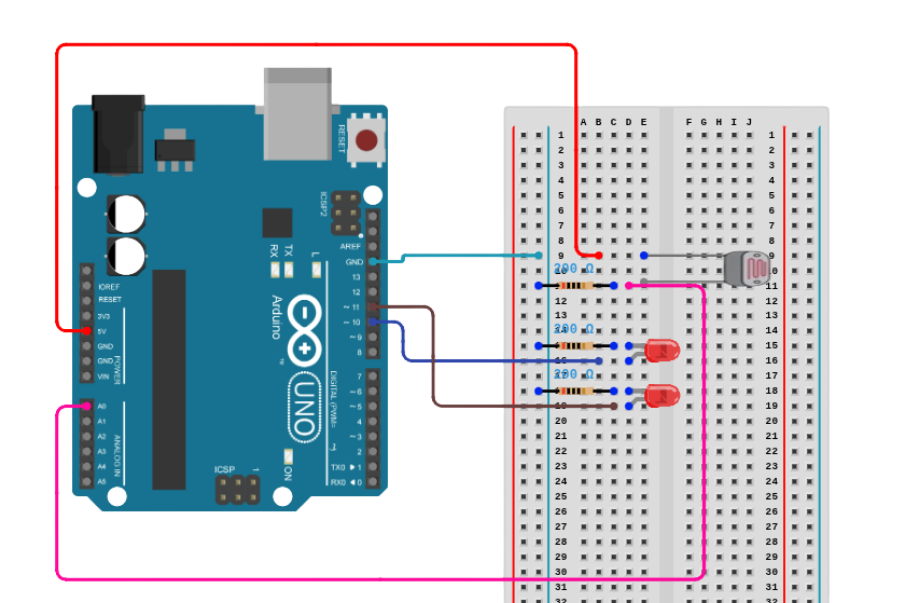
\includegraphics[width=\linewidth]{Image/2.Schéma_Manip3}
		\caption{Schéma du montage avec photorésistance et deux LED}
		\label{fig:schema_photores}
	\end{minipage}\hfill
	\begin{minipage}{0.48\textwidth}
		\centering
		\includegraphics[width=\linewidth]{Image/2.Photo_Manip3}
		\caption{Photo montage avec la photorésistance et deux LED}
		\label{fig:photo_photores}
	\end{minipage}
\end{figure}
\begin{lstlisting}					
void loop() {	
	sensorValue = analogRead(analogInPin);
	
	outputValue = map(sensorValue, 0, 1023, 0, 255);
	
	analogWrite(analogOutPin, outputValue);
	
	Serial.print("sensor = " );
	Serial.print(sensorValue);
	Serial.print("\t output = ");
	Serial.println(outputValue);	
	if(sensorValue < ((1023*1)/100) ){
		digitalWrite(11, HIGH);
	}else{
		digitalWrite(11, HIGH);
	}	
}
\end{lstlisting}
\textbf{Observations :} Les deux LED s'allume bien lorsque en fonction du seuil de luminosité atteint.
\section{Variation de la luminosité d'une LED avec un potentiomètre et une carte Arduino}
Pour terminer cette manipulation, nous intégrons un potentiomètre au lieu d'un capteur automatique. Cela nous donne la possibilité de contrôler manuellement le circuit en modifiant la valeur de sa résistance.
\begin{figure}[H]
	\centering
	\begin{minipage}{0.48\textwidth}
		\centering
		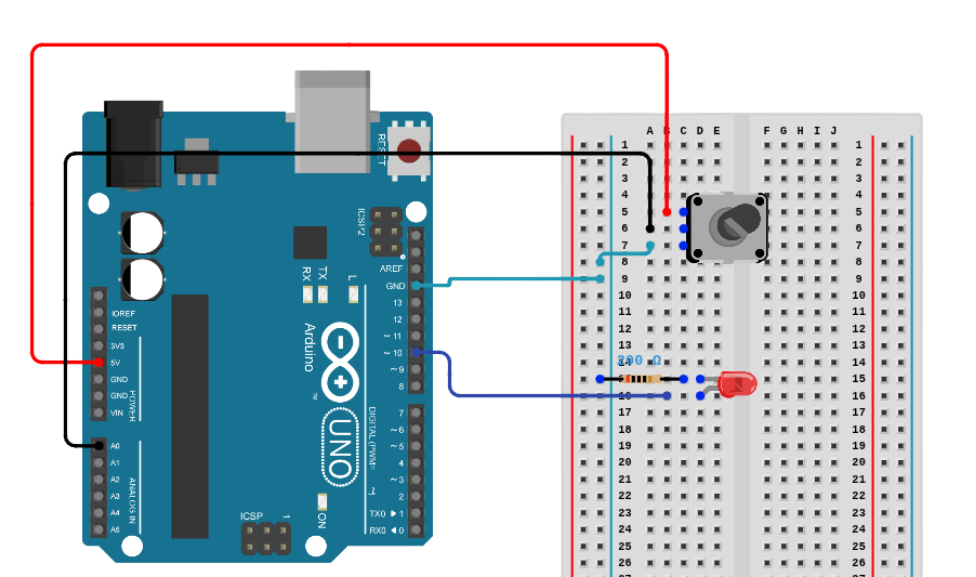
\includegraphics[width=\linewidth]{Image/2.Schéma_Manip4}
		\caption{Schéma du montage avec le potentiomètre}
		\label{fig:schema_photores}
	\end{minipage}\hfill
	\begin{minipage}{0.48\textwidth}
		\centering
		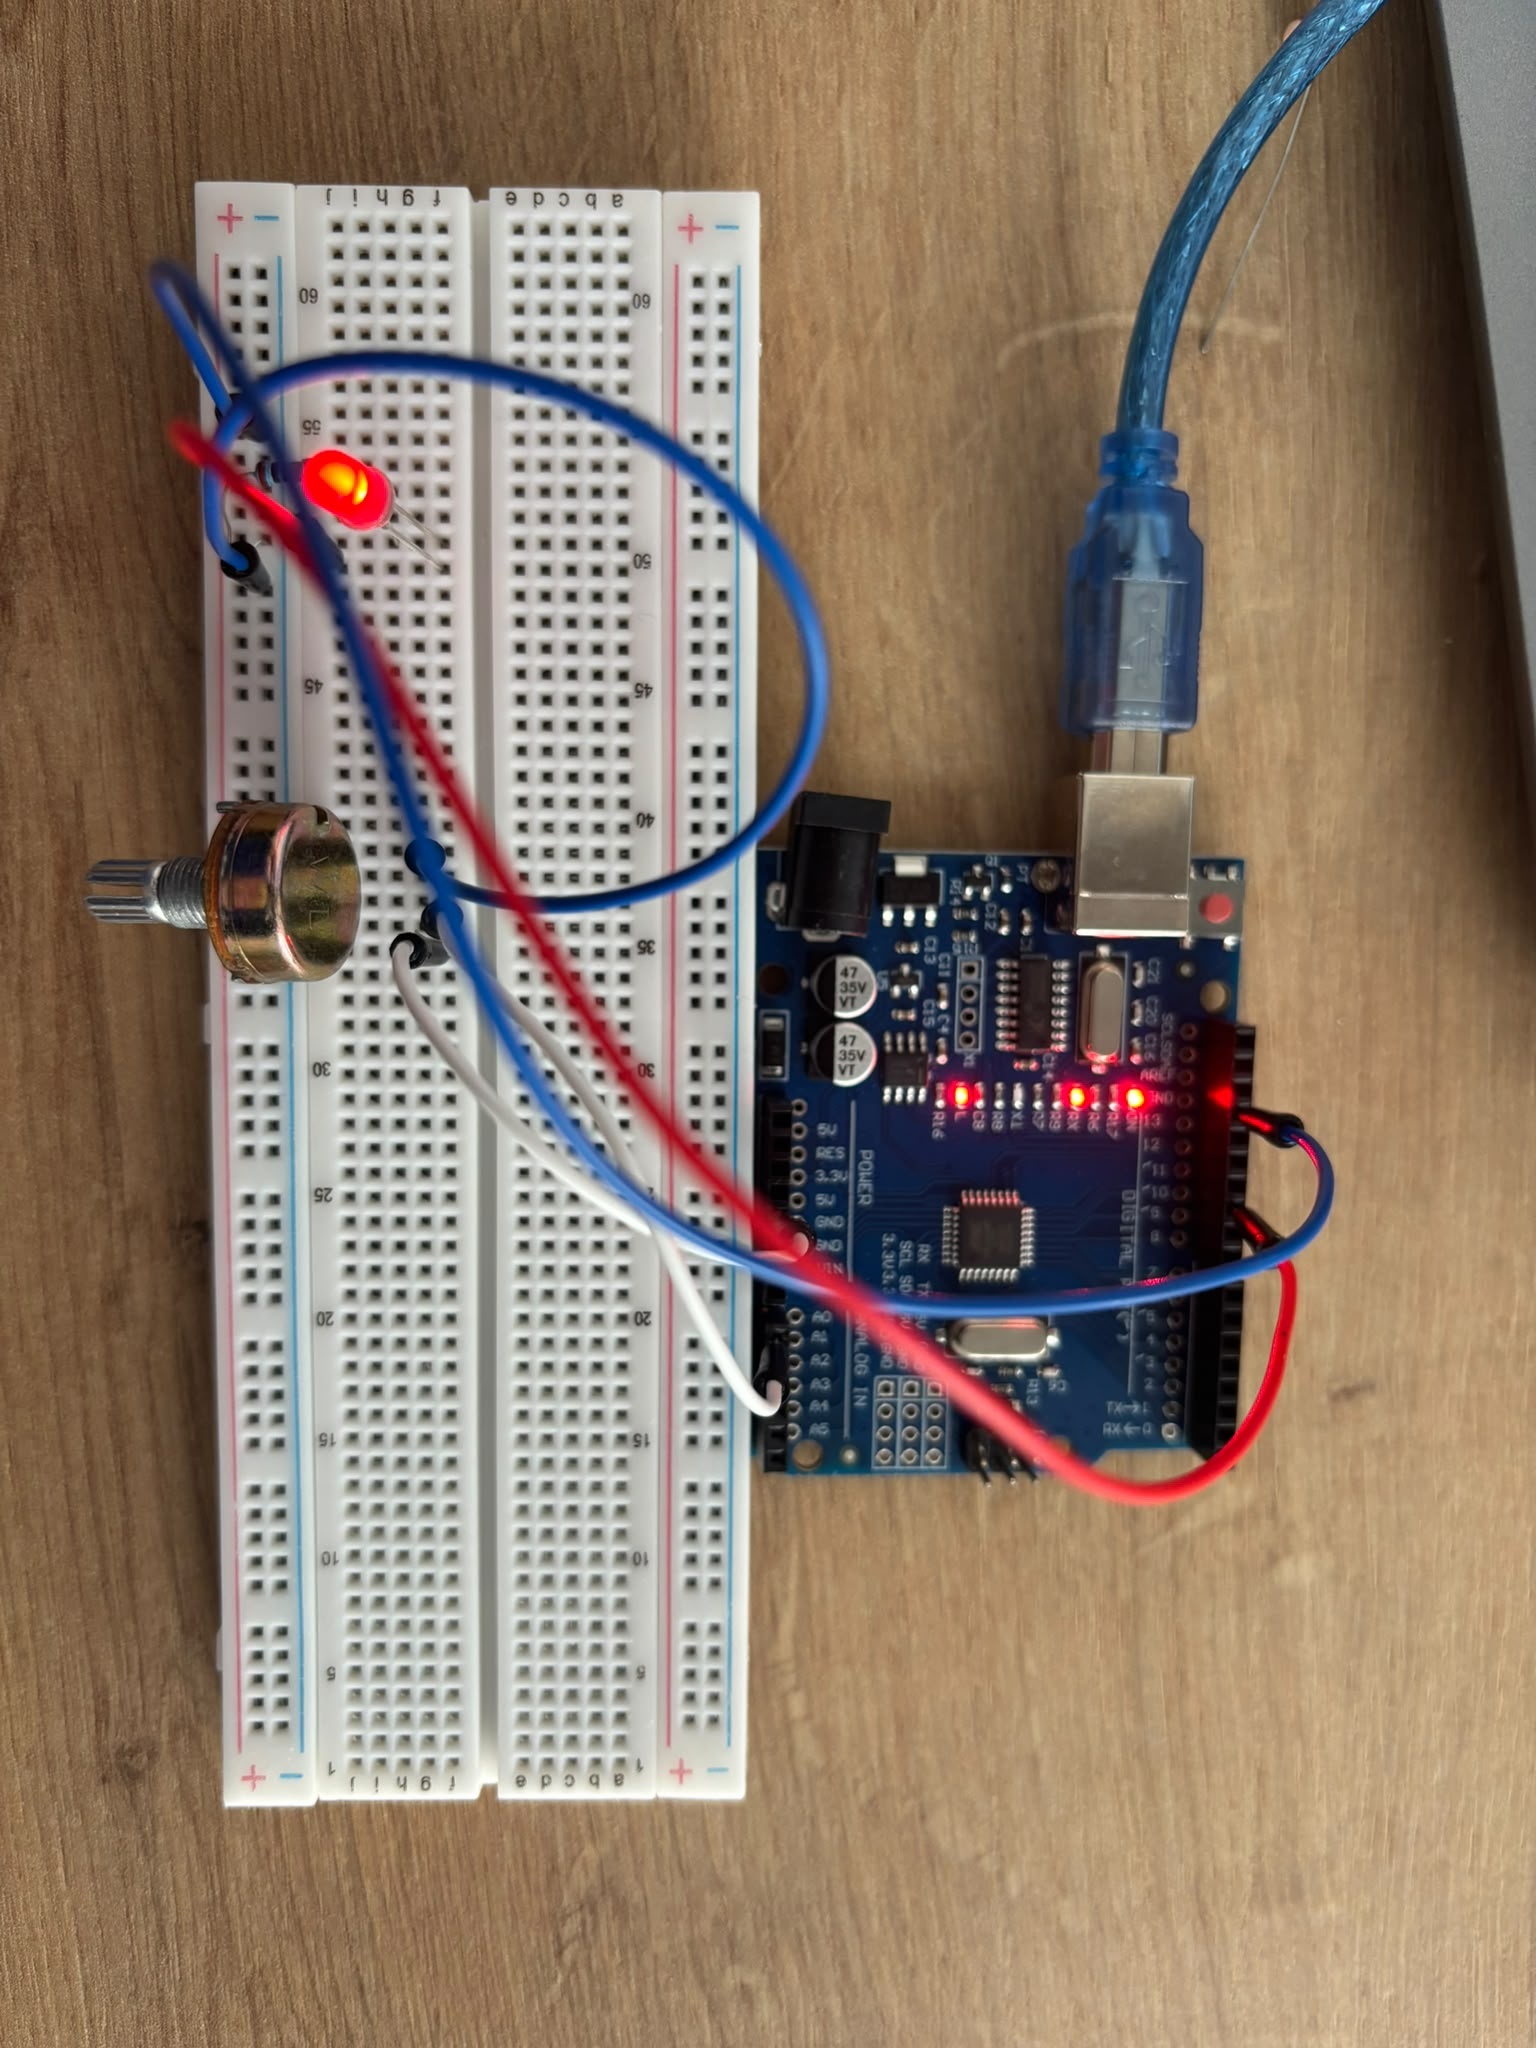
\includegraphics[width=\linewidth]{Image/2.Photo_Manip4}
		\caption{Photo montage avec le potentiomètre}
		\label{fig:photo_photores}
	\end{minipage}
\end{figure}
Nous modifions alors un peu le code de la photorésistance pour utiliser le potentiomètre.
\begin{lstlisting}					
	void loop() {
		
		sensorValue = analogRead(analogInPin);
		
		outputValue = map(sensorValue, 0, 1023, 0, 255);
		
		analogWrite(analogOutPin, outputValue);
		
		Serial.print("sensor = " );
		Serial.print(sensorValue);
		Serial.print("\t output = ");
		Serial.println(outputValue);		
	}	
\end{lstlisting} 
\textbf{Observations :} La LED s'allume bien lorsque que nous tournons le potentiomètre.\\
Nous ajoutons ensuite une autre LED qui devras s'allumer quand le potentiométre est au minimum.
\begin{figure}[H]
	\centering
	\begin{minipage}{0.48\textwidth}
		\centering
		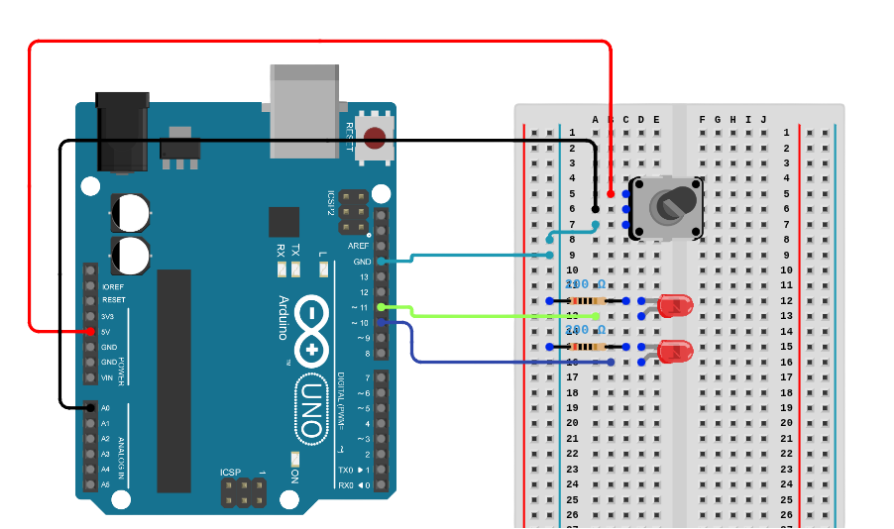
\includegraphics[width=\linewidth]{Image/2.Schéma_Manip5}
		\caption{Schéma du montage du potentiométre avec 2 LED}
		\label{fig:schema_photores}
	\end{minipage}\hfill
	\begin{minipage}{0.48\textwidth}
		\centering
		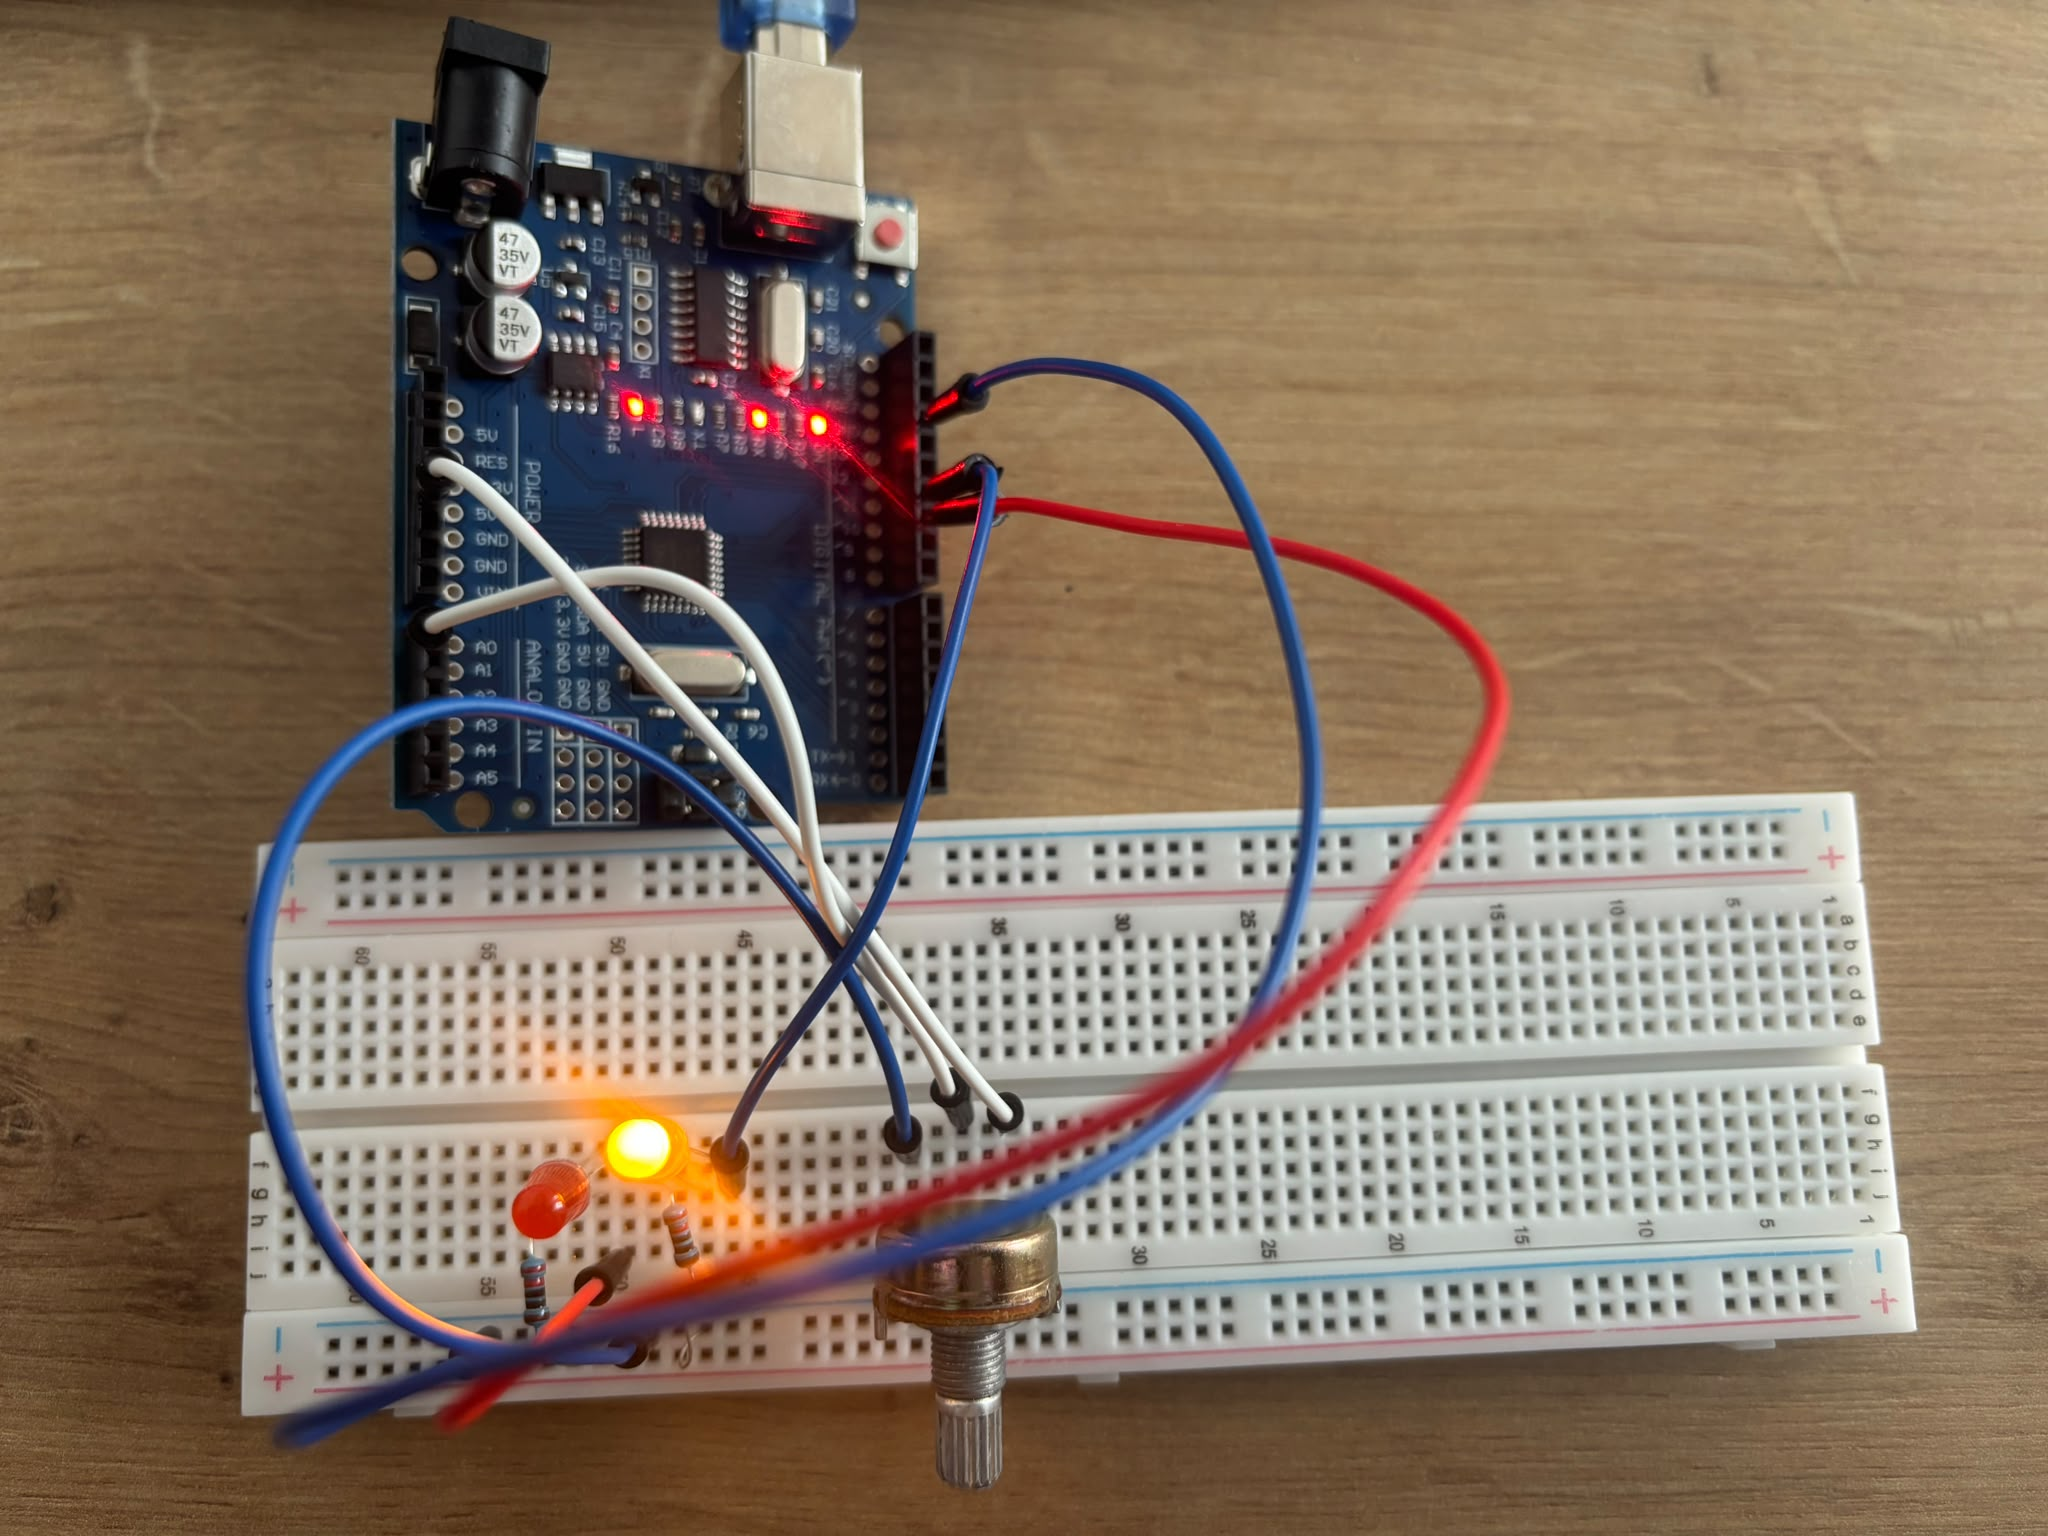
\includegraphics[width=\linewidth]{Image/2.Photo_Manip5}
		\caption{Photo montage du potentiométre avec 2 LED}
		\label{fig:photo_photores}
	\end{minipage}
\end{figure}
\begin{lstlisting}					
	void loop() {
		
		sensorValue = analogRead(analogInPin);
		
		outputValue = map(sensorValue, 0, 1023, 0, 255);
		outputValue2 = map(sensorValue, 0, 1023, 255, 0); // on inverse le 255
		
		analogWrite(analogOutPin, outputValue);
		analogWrite(11, outputValue2);
		
		Serial.print("sensor = " );
		Serial.print(sensorValue);
		Serial.print("\t output = ");
		Serial.println(outputValue);
			
	}
	
\end{lstlisting} 
\textbf{Observations :} Tourner le potentiomètre dans un sens allume une première LED, le tourner dans l'autre sens allume la seconde.\\
Pour finir avec ce TP nous devons afficher sur un écran LCD la température que nous mesurons a l'aide du LM35 utilisé dans la première partie du TP.
Pour ce faire nous utilisons un code qui a été fournie par une bibliothèque trouvé sur Google.
\begin{lstlisting}					
	#include <Wire.h>
	#include <LiquidCrystal_I2C.h>	
	const int lm35Pin = A0; // Broche du capteur LM35	
	// Initialisation du LCD I2C : Adresse 0x27, 16 colonnes, 2 lignes
	LiquidCrystal_I2C lcd(0x27, 16, 2); 
	
	void setup() {
		// Initialisation du LCD
		lcd.init();
		lcd.backlight(); // Allume le retroeclairage
		lcd.clear();
	}	
	void loop() {
		int val = analogRead(lm35Pin); // Lecture du capteur
		
		// Conversion en temperature (C)
		float voltage = val * (5.0 / 1023.0);
		float temperature = voltage * 100.0; 
		
		// Affichage sur l'ecran LCD
		lcd.setCursor(0, 0); // Ligne 1
		lcd.print("Temp: ");
		lcd.print(temperature, 1); // 1 chiffre apres la virgule
		lcd.print(" C   "); // Espaces pour eviter les bugs d'affichage
		
		delay(1000); // Pause d'une seconde avant la prochaine mesure
	}	
\end{lstlisting}  
\begin{figure}[H]
	\centering
	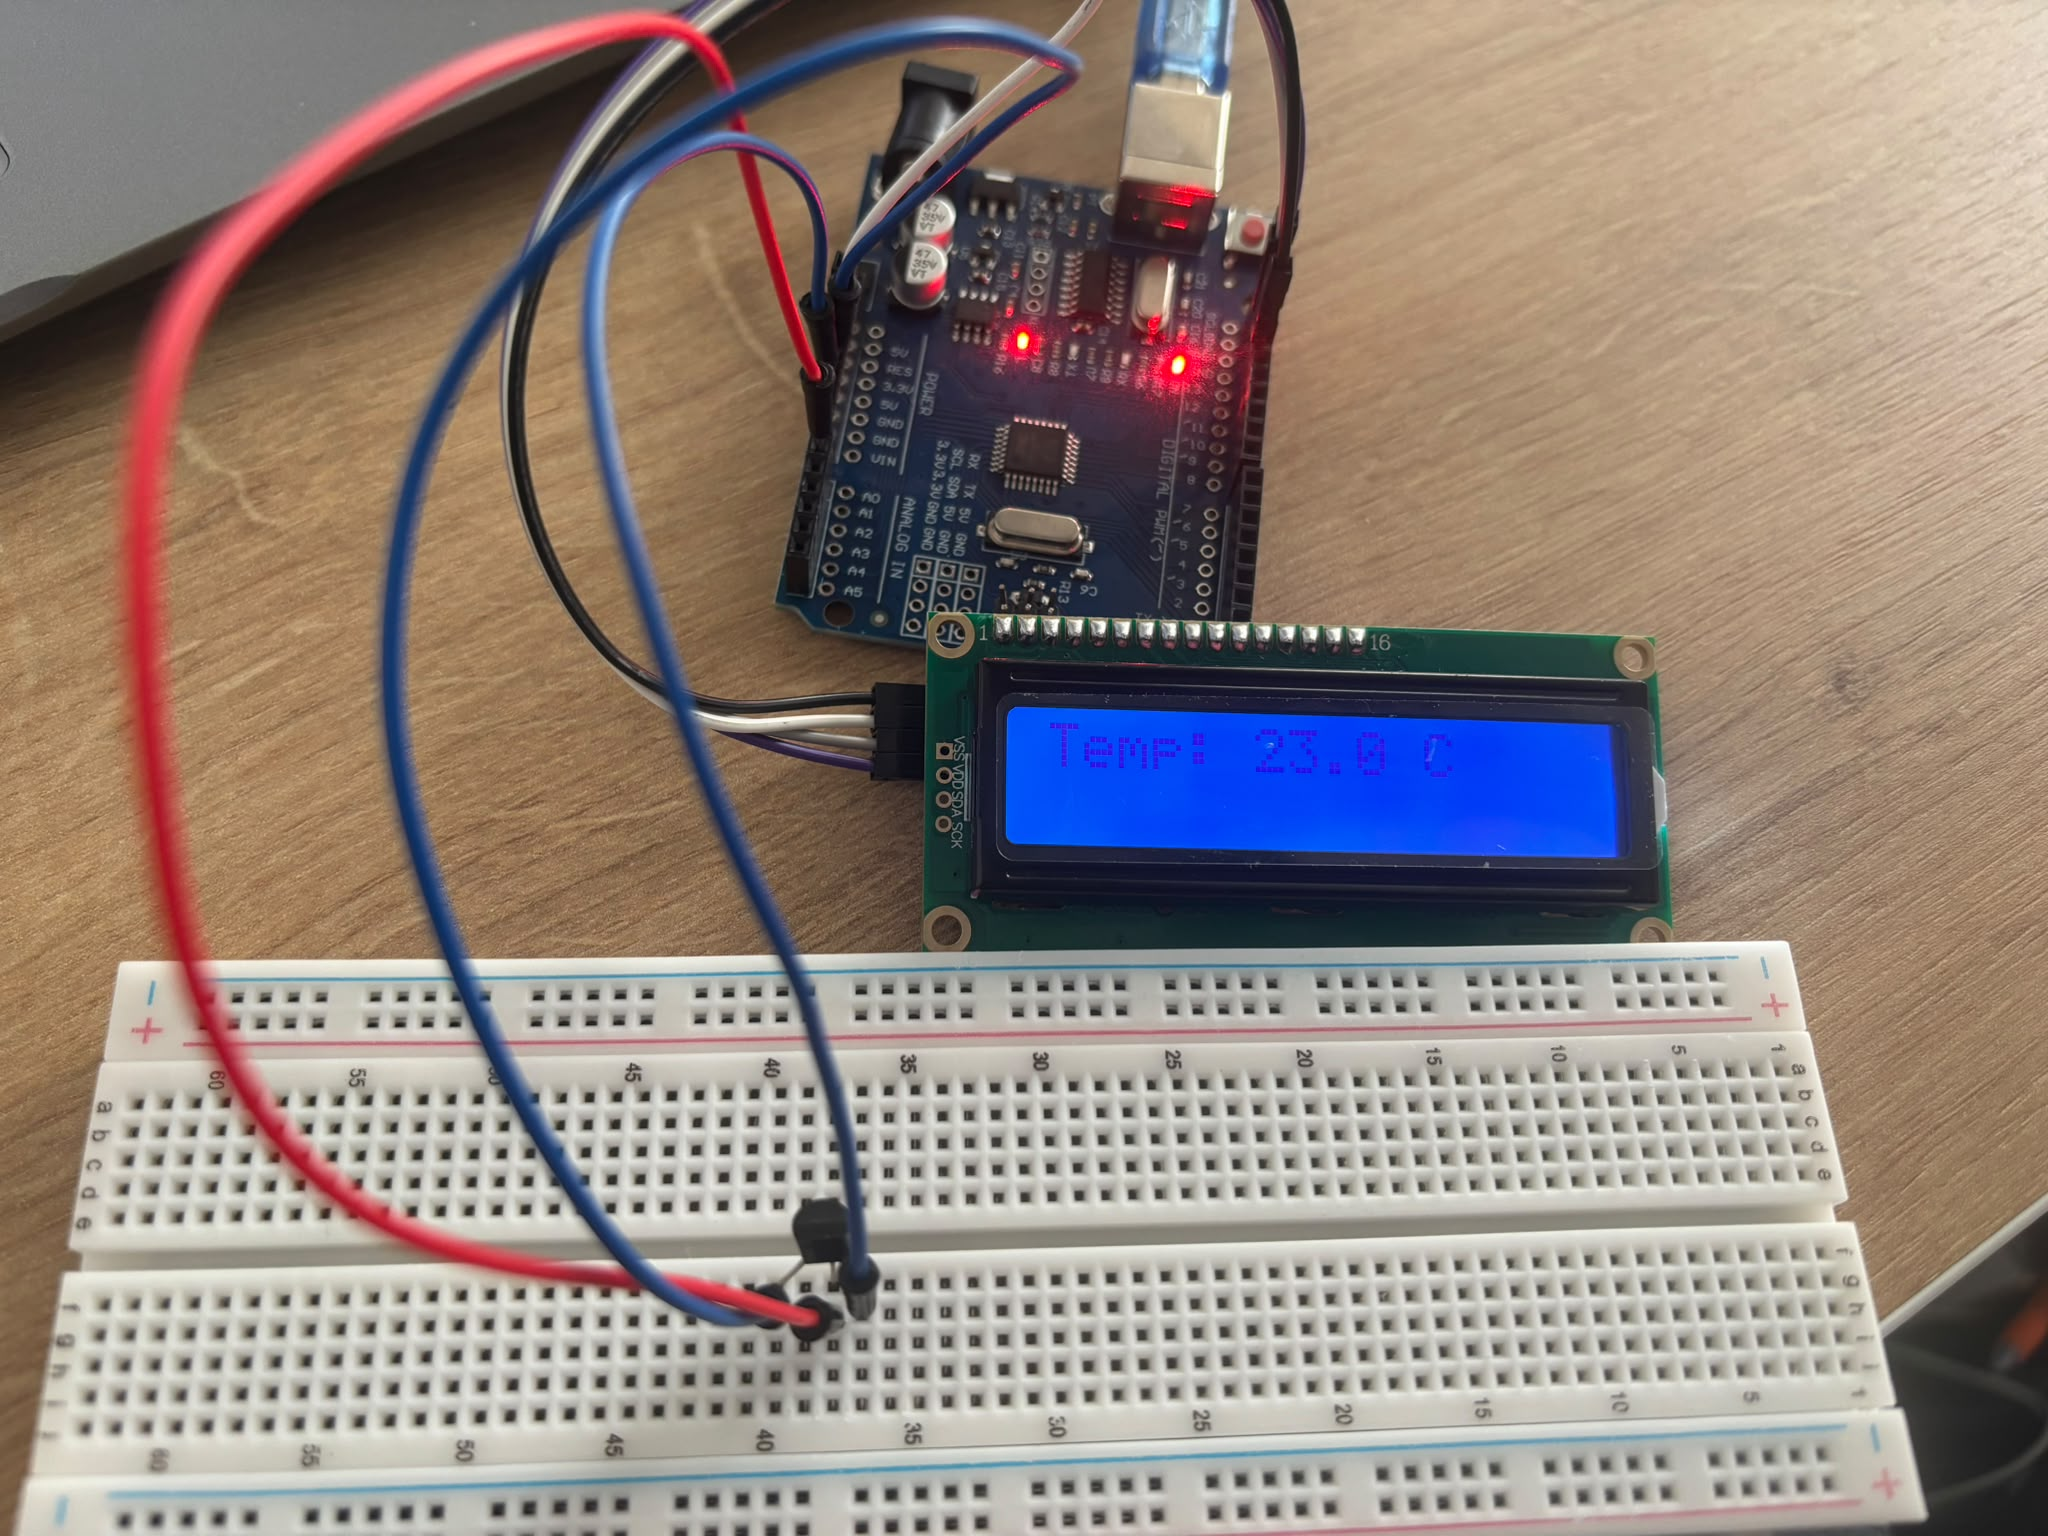
\includegraphics[width=0.7\linewidth]{Image/Photo_manip6}
	\caption{Montage de l'affichage sur l'écran LCD}
	\label{fig:photomanip6}
\end{figure}
